\chapter{Introduction}
The Final Year Project, a chance for myself to culminate what i have learned in the four years of study in the field of software development to produce the project of my choosing. When choosing what i wanted to develop for my final year project, i had to split it up in to many different aspects. The idea, the reasoning and why it would be beneficial for human use and also economically sufficient for the target audience. I also needed to choose a technology to use, what programming language will i use, pros and cons, what database storage will i use to store data applicable to what i will develop.  

\begin{figure}[h!]
	\caption{Various Software Languages to choose from.}
	\label{image:progLanguages}
	\centering
	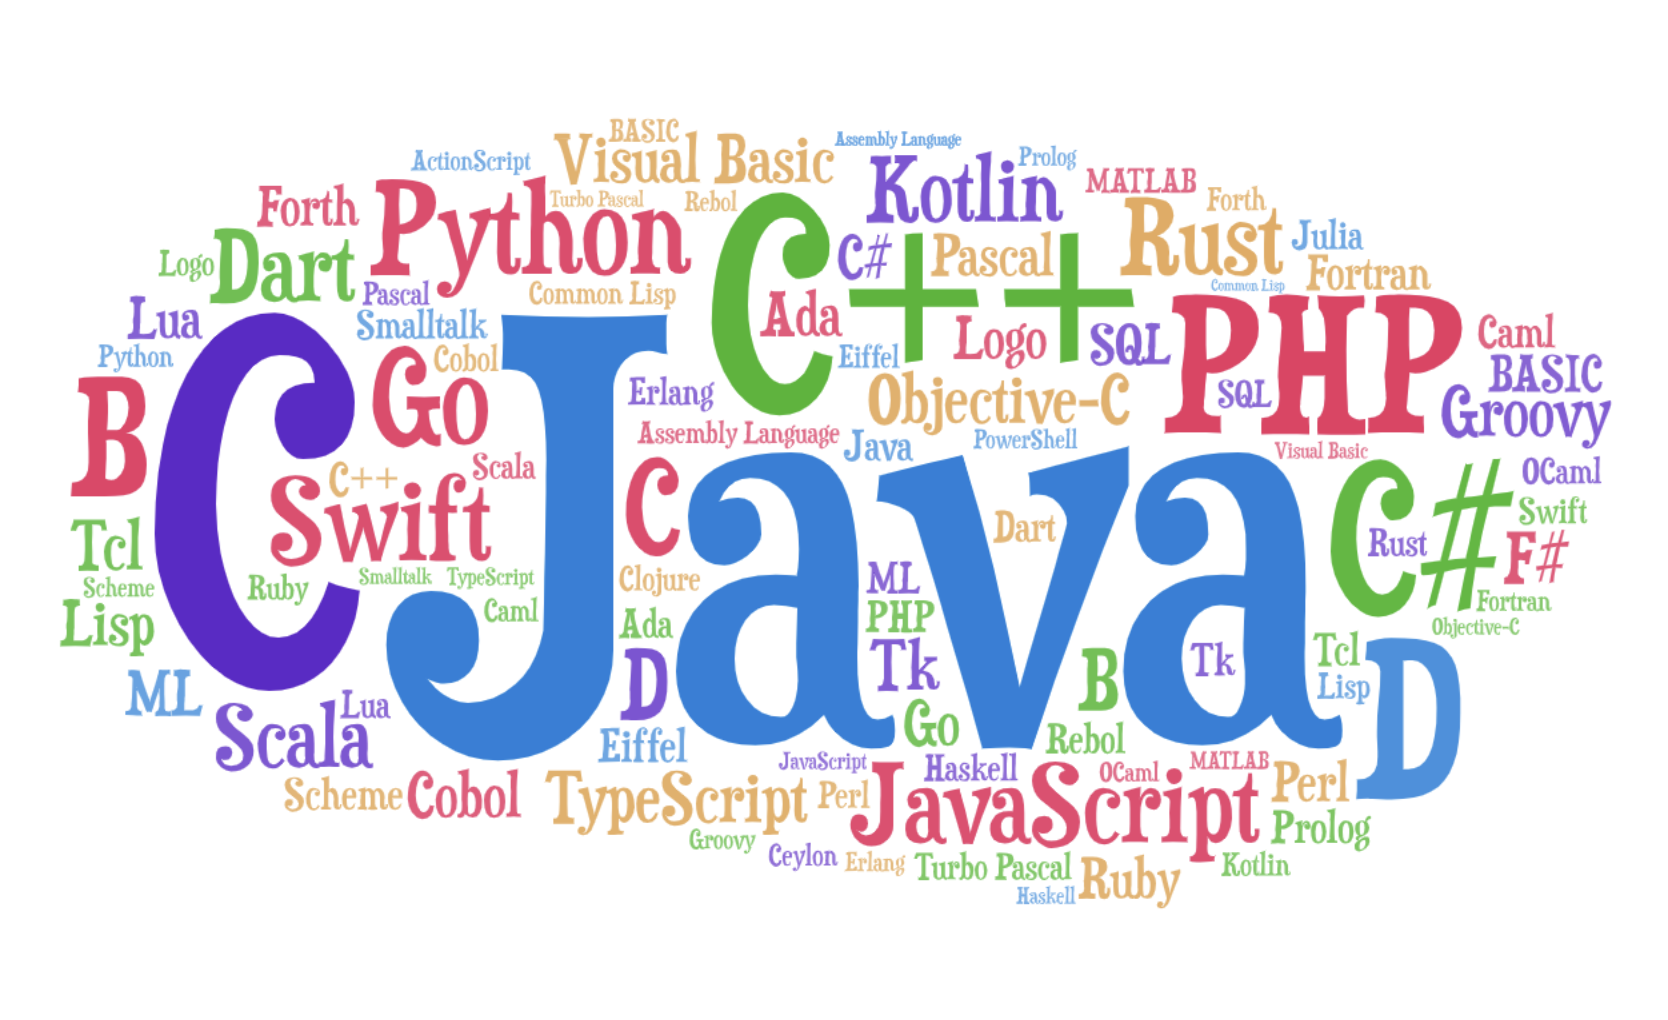
\includegraphics[width=0.8\textwidth]{images/progLanguages.png}
\end{figure}	

\newpage

When deciding on what type of project and application to pursue, i wanted to integrate it into something involved in my weekly life. My part time job as a Sales Assistant benefited me in making a decision on what type of project to do. I looked into the everyday functionality of the shop and after working there for just under 5 years i was very experienced in knowing the day to day operations of the store. I looked at different ways i can make the staffs job easier and at the same time, save the shop money by creating this application. I also used Google Scholars to gather more information on this problem in retail and will be referencing the citations throughout the dissertation. Here is a article citation that gave information about the amount of food loss in the industry and the problem i wish to solve with this application is to reduce this number by getting to a product in time to use elsewhere in the store such as the deli or even reduce the item. \cite{lebersorger2014food}
\newline

When deciding on a technology to use, i wanted to use what suited me for the system design and development stage. I wanted to choose a database for data storage that i was familiar with and what made my life easier. What IDE will i use to code my project. There were so many available but ultimately i chose the one that suited me and the project combined. I also needed to pick a database service to work of, Amazon Web Service (AWS), Firebase, MongoDB and Microsoft Azure all come to mind as during this course i encountered all of these some for assignments and some for personal projects which i have done during the tenure of this course. I had a decision to make, the decision had to make sense for me and for the project itself, what elements of each would benefit me and the functionality of the software development.
\newline

\begin{figure}[h!]
	\caption{Database Option: Firebase.}
	\label{image:firebase}
	\centering
	
\includegraphics[width=0.3\textwidth]{images/firebase.png}
\end{figure}

\begin{figure}[h!]
	\caption{Database Option: MongoDB.}
	\label{image:mongodb}
	\centering
	
\includegraphics[width=0.3\textwidth]{images/mongodb.png}
\end{figure}

\newpage

\begin{figure}[h!]
	\caption{Database Option: Microsoft Azure.}
	\label{image:azure}
	\centering
	
\includegraphics[width=0.3\textwidth]{images/azure.png}
\end{figure}

\begin{figure}[h!]
	\caption{Database Option: Amazon Web Service (AWS).}
	\label{image:aws}
	\centering
	
\includegraphics[width=0.3\textwidth]{images/aws.png}
\end{figure}


I wanted to create something that would help my workplace, my fellow staff members and of course my management team and saving time and money for the shop I've been working in for five years. I noticed one element that is being done but not everything catches the eye. Date Control. This is obviously observed by the retail staff who work on the shop floor, who go around and check the products best before date.  This is obviously done in a manual manner and due to uncontrollable human error of missing a product and not to mention the stock room barley being checked I've come up with the idea of producing a application/program that allows the staff member to look at this application to see every product for each section of the shop such as biscuits and cakes section, dairy, meats and so on and being able to identify which items to take off the shelf and either scan them for returns, reduce the items or waste them, depending on the type of product and the safety of selling that particular product.   
\newline

I decided to pursue this project as i feel it links my college life and work experience together as one. When picking my technologies to produce this project i looked at every aspect of each technology however after much thought and looking at the pros and cons for each, i decided to develop this project inevitably in ionic Firebase. I had past experience for both and being honest had the best experience of both, i like the way it both connect and the smoothness of ionic when coding and running. This was not my initial pick, which i will mention later on in this dissertation.

\begin{figure}[h!]
	\caption{Chosen Technology for Date Control Application, Ionic Firebase.}
	\label{image:ionicfirebase}
	\centering
	
\includegraphics[width=0.4\textwidth]{images/ionicfirebase.png}
\end{figure}

\newpage

\begin{figure}[h!]
	\caption{Best Before Date Example Fig.}
	\label{image:bbdate}
	\centering
	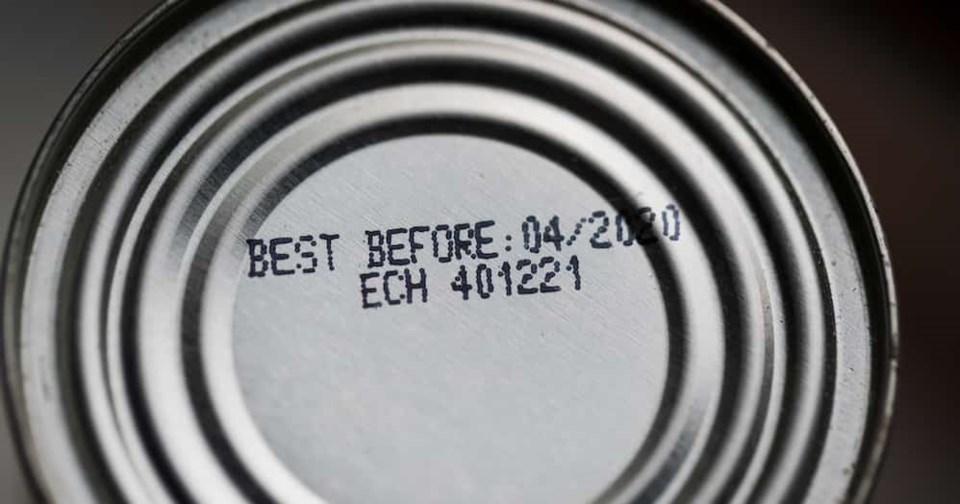
\includegraphics[width=0.3\textwidth]{images/bbdate.jpg}
\end{figure}

In this dissertation i will be covering every aspect of this project including the following:
\newline 

- The Methodology of the project, the software development and research side of the project, the type of approach made to development, the testing of the project, the development tools and the usage of GitHub.
\newline

- The Technology Review, why i pursued this project, why did i want to help my workplace, is my project idea beneficial and sufficient, surveys conducted, the planning of the project basically my developer diary, technologies used in the project even extra ones if any, the references used in helping me develop the software application, the issues and limitations encountered during the software development and any other elements i didn't mention.
\newline

- The System Design, how i designed it, styling and HTML etc., the design sketches i did for the application, what i wanted my program to look like and why i designed it like i did, and of course any extras i learned when developing the design of the application.
\newline

- The System Evaluation, the objectives and goals set out, were they achievable ?, the software testing results shown in a testing excel sheet, results of the conducted surveys, testing conducted by my fellow staff members, and the limitations i had for this project.
\newline

- The Conclusion, where i will look back at the rationale and goals of the overall project, i will highlight my findings from my system evaluation and discuss the opportunities and flexibility this project has made for me and others especially the target audience, can it do more than one thing, can it benefit me for future interviews and could i possibly present this idea to potential investors etc.
\newline

- The References and Appendices, here i will include my GitHub repository for the software development of the application for the project and the references i used to help me develop the application and give a brief description for each reference. It will also include how to run the application accordingly.
\newline

- The Bibliography, here i will include in articles, pieces or reference to a quotation from it's citation. This is the information i gained in my research on this particular product of date control in retail. 
\newpage

\begin{figure}[h!]
	\caption{GitHub Containing the Software Application for the Project.}
	\label{image:github}
	\centering
	
\includegraphics[width=0.7\textwidth]{images/github.png}
\end{figure}

The GitHub Repository i used to commit and push my software development accordingly is: https://github.com/AndreasFahey/AppliedProject-DateControl
\newline

Here you will find all my work both in researching and development of the project and how to download and run the application. You will also see issues raised during the project and if they were resolved. Also the commits and what i done for each commit will also be available to see the timeline in which i did things in the software development side of the project. This full dissertation will also be available on the GitHub repository as part of the download of the project along with a screen cast, PowerPoint and software testing results on a excel document.



